  Durch eine Detailanalyse der Aufgabenstellung werden die wichtigsten
  Aufgaben und deren Resultate ausgearbeitet. Aufgrund dieser Erkenntnisse
  wird eine Grobplanung festgelegt. Damit die Nachvollziehbarkeit garantiert
  ist, werden die Termine, Meilensteine und Arbeitsschritte aufgelistet.
  
  \section{Detailanalyse der Aufgabenstelltung}
  
  \indent
  \indent
  ``\begin{itshape}Analyse bestehender Java Swing Applikationen der Zürcher
  Kantonalbank.\end{itshape}''
  \newline
  \newline
  \noindent
  Es sollen die gängigen Mechanismen von Java Swing Applikationen der Zürcher
  Kantonalbank untersucht werden, dass soll aus der Sicht des Anwenders
  passieren. In drei bestehenden Java Swing Applikationen soll die Existenz
  bekannter GUI Paradigmen untersucht werden.
  \newline
  \newline
  \noindent
  Resultat: Es soll eine Liste der erkannten Paradigmen vorliegen.
  \newline
  
  ``\begin{itshape}Erkennen und Kategorisieren der verwendeten
  Swingkomponenten.\end{itshape}''
  \newline
  \newline
  \noindent
  Die drei ausgewählten Java Swing Applikationen werden genauer betrachtet. Es
  wird das Augenmerk auf die Verwendung von Swingkomponenten gelegt. Diese
  sollen über die drei Applikationen hinweg konsolidiert und kategorisiert
  werden.
  \newline
  \newline
  \noindent
  Resultat: Es soll eine Liste der verwendeten Swingkomponenten vorliegen.
  \newline
  
  ``\begin{itshape}Evaluation von Java Web Frameworks, welche sich am Markt
  etabliert haben.\end{itshape}''
  \newline
  \newline
  \noindent
  Es soll ein Evaluationsverfahren gewählt werden, bei dem eine möglichst
  objektive Entscheidung gefällt werden kann. Welche Java Web Frameworks in die
  Evaluation miteinbezogen werden, soll über Recherchen im Internet und in
  Büchern geschehen. Es sollen fünf Java Web Frameworks gewählt werden, welche
  anhand der Recherchen für valable Optionen in Frage kommen. Über die
  Definition von Soll- und KO-Kriterien sollen die Rahmenbedigungen für das
  Evaluationsverfahren geschaffen werden. Anhand der ausgearbeiteten
  Evalautionsmethode soll gezeigt werden, wie geeignet die Java Web Frameworks
  wirklich sind.
  \newline
  \newline
  \noindent  
  Resultat: Es soll eine Rangliste der fünf Frameworks, in der Anordnung
  entsprechend ihrer Eignung, vorliegen.
  \newline

  ``\begin{itshape}Prüfen, ob eine Integration der evaluierten Java Web
  Frameworks, welche für eine Umsetzung geeignet sind, in der bestehenden IT
  Infrastruktur der Zürcher Kantonalbank möglich ist.\end{itshape}''
  \newline
  \newline
  \noindent
  Gemäss den Vorgaben der IT Infrastruktur der Zürcher Kantonalbank, soll ein
  mögliche Einsatz der evaluierten Java Web Frameworks geprüft werden. Die
  meisten Java Web Frameworks haben in ihrer Dokumentation die Anforderungen
  definiert, welche für einen möglichen Betrieb nötig sind. Aufgrund dieser
  Anforderungen, und der bestehenden IT Infrastruktur soll ein Vergleich gemacht
  werden.
  \newline
  \newline
  \noindent
  Resultat: Es sollen die Java Web Frameworks aufgelistet werden, welche für
  einen Einsatz in der IT Infrastruktur der Zürcher Kantonalbank in Frage kommen.
  \newline

  ``\begin{itshape}Prüfen, ob eine Implementierung der erkannten
  Swingkomponenten in den evaluierten Java Web Frameworks möglich
  ist.\end{itshape}''
  \newline
  \newline
  \noindent
  Die gewonnenen Erkenntnisse, aus der Analyse der Java Swing Applikationen,
  sollen nun mit der Liste, der in Frage kommenden Java Web Frameworks,
  zusammengeführt werden.
  \newline
  \newline
  \noindent
  Resultat: Es sollen die Java Web Frameworks aufgelistet werden, welche die
  notwendigen Swingkomponenten und GUI Paradigmen unterstützen.
  \newline

  ``\begin{itshape}Proof of concept. Erstellen eines Prototypen mit den
  evaluierten Java Web Frameworks und den erkannten
  Swingkomponenten.\end{itshape}''
  \newline
  \newline
  \noindent
  Das Java Web Framework, welches sich entsprechend der Evaluation am meisten
  für den Einsatz eignet und den Anforderungen der IT Infrastruktur und der
  notwendigen Swingkomponenten und GUI Paradigment genügt, soll sich anhand
  eines definierten Prototypen bewähren.
  \newline
  \newline
  \noindent
  Resultat: Es soll eine Empfehlung eines Java Web Frameworks, für den
  möglichen Einsatz in der Zürcher Kantonalbank, ausgesprochen werden.
  
  \section{Grobplanung}
  
  Die Grobplanung sieht man anhand der Grafik \ref{grobplanung}:
  
  \begin{figure}[h]
    \begin{center}
      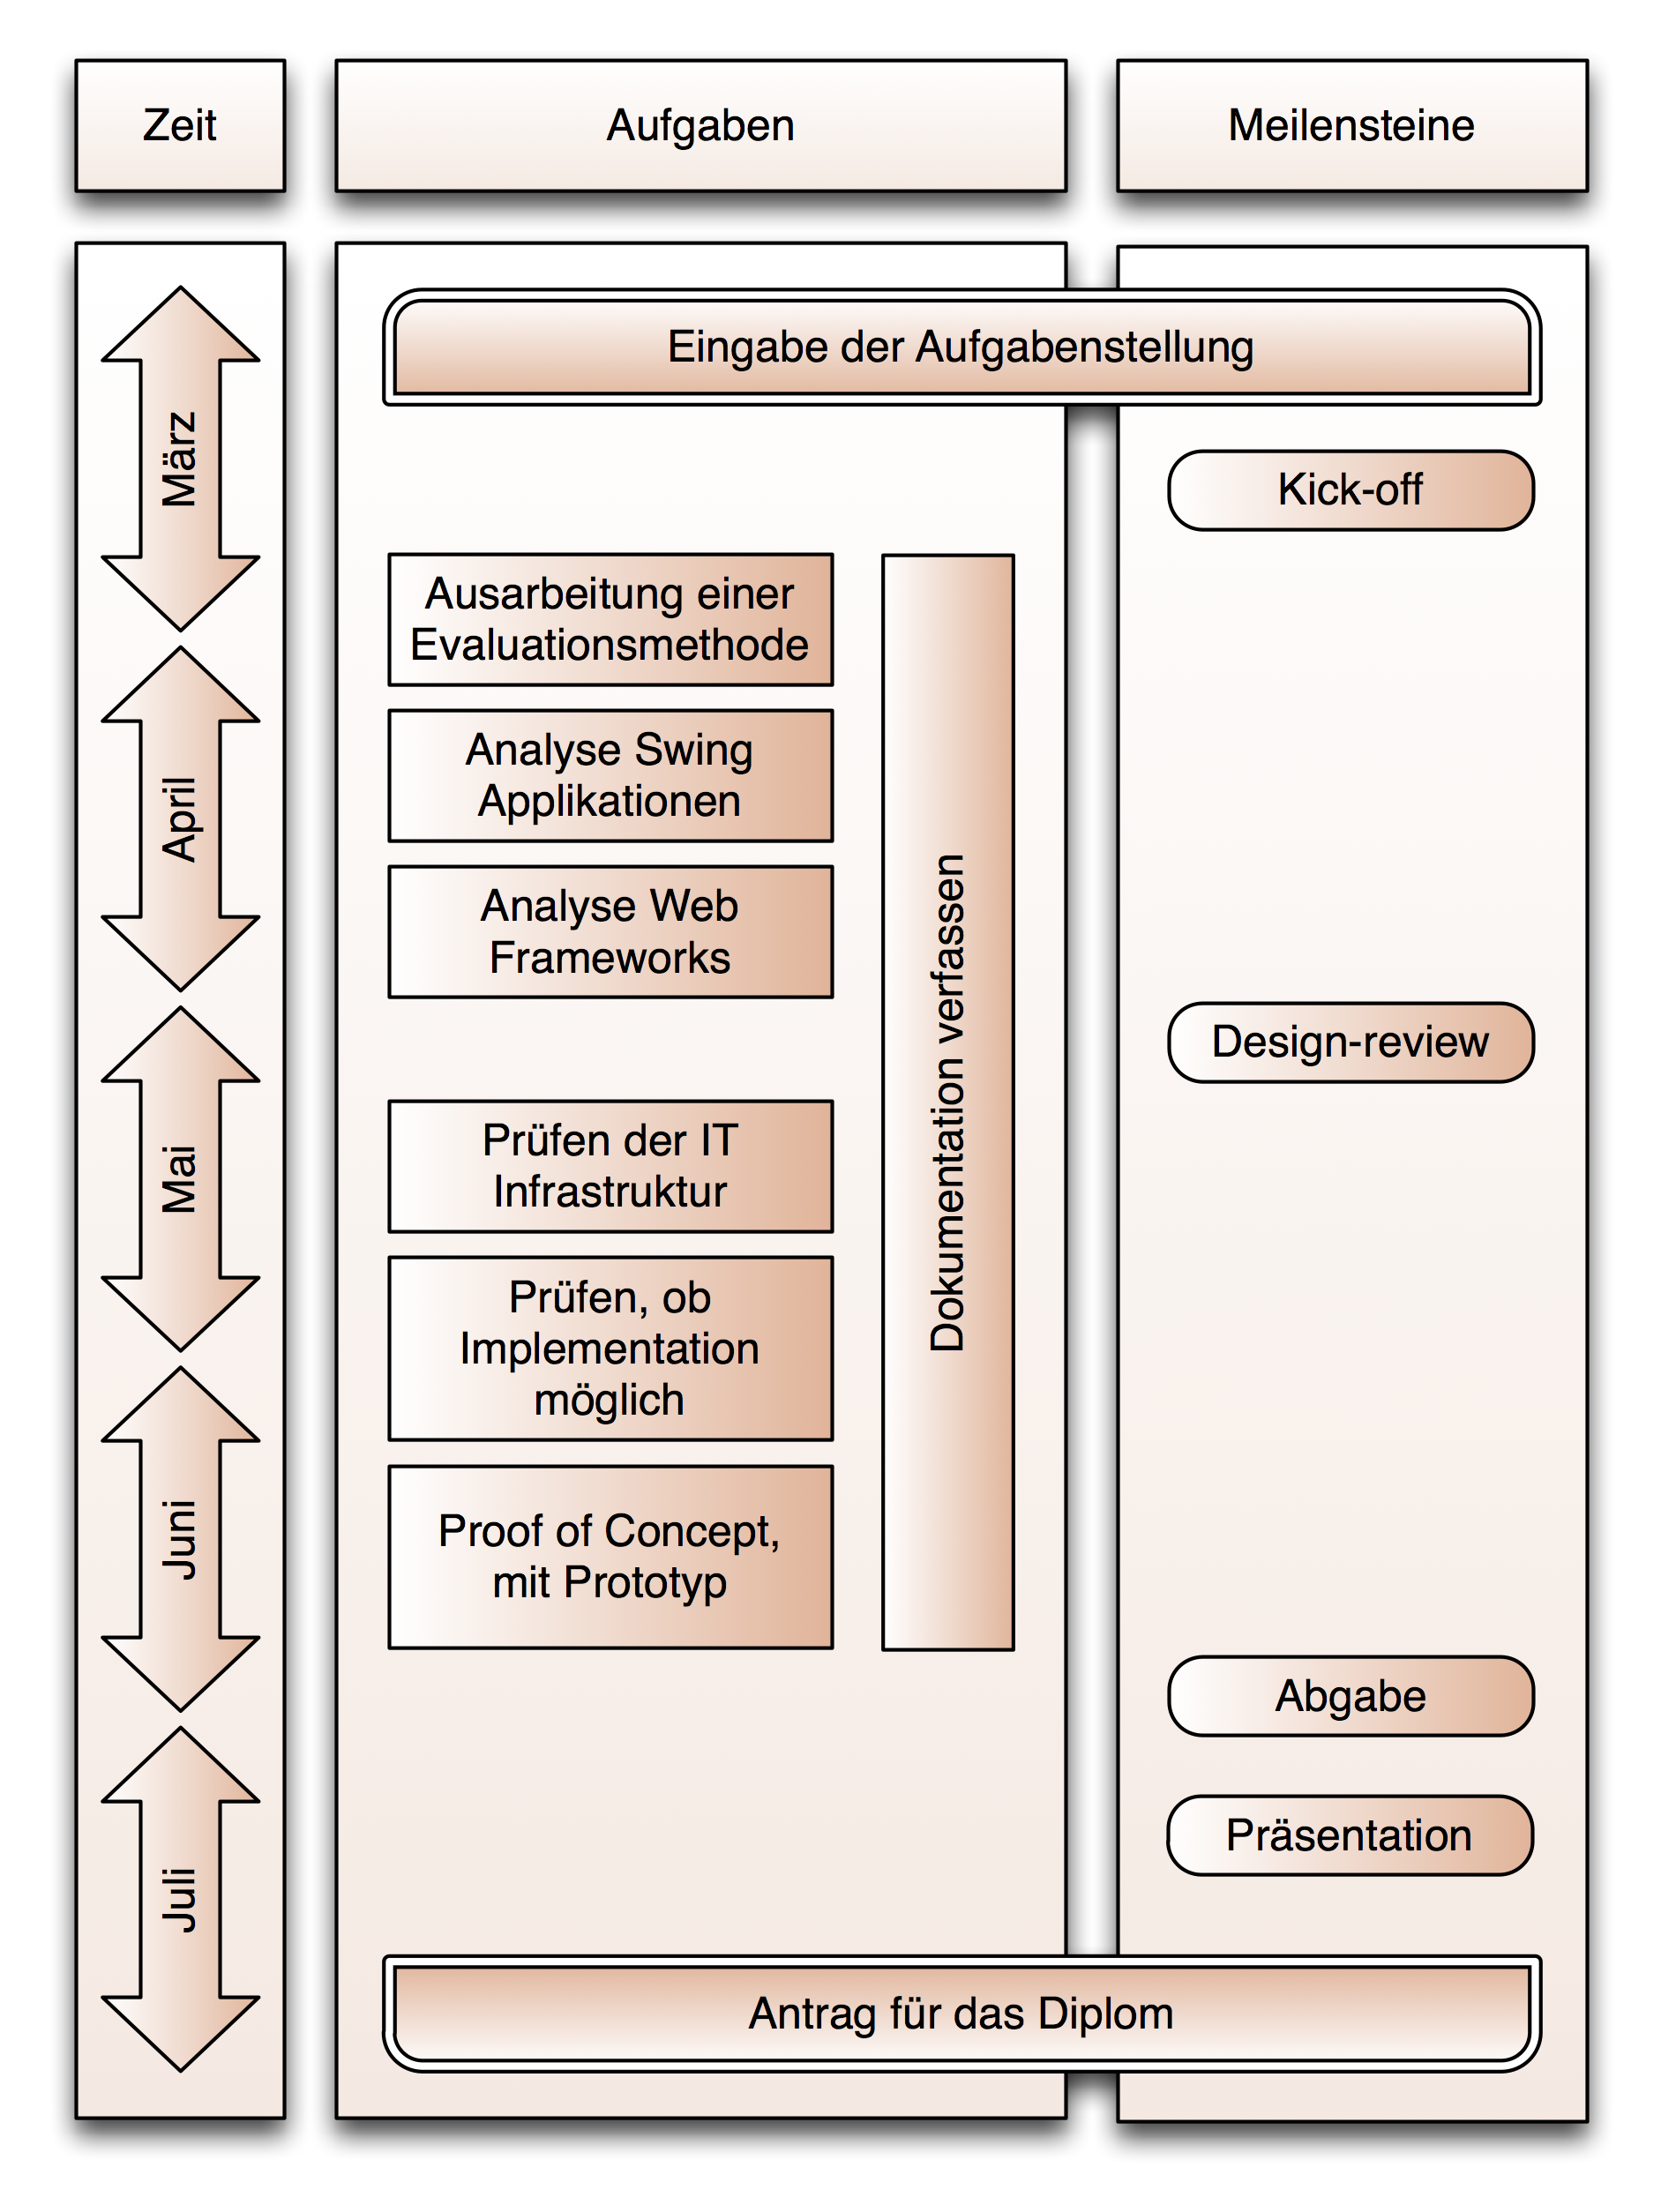
\includegraphics[width=0.7\textwidth]{./image/grobplanung.png}
      \caption{Grobplanung zur Diplomarbeit}
      \label{grobplanung}
    \end{center}
  \end{figure}
  
  \section{Termine}
  
  Die Projekt Termine wurden alle eingehalten, siehe Tabelle \ref{tab:termine}.
  \newline
  
  \begin{table}[h]
    \begin{center}
      \begin{tabular}{lp{7cm}ll}
        \toprule
        Termin & Datum & Ort \\
        \midrule
        21. 03. 2011 & Inhaltliches Kick-off Meeting & Panter llc\\
        13. 04. 2011 & Offizielles Kick-off Meeting & HSZ-T\\
        xx. xx. 2011 & Design-Review Meeting & HSZ-T\\
        xx. xx. 2011 & Abgabe der Dokumentation & HSZ-T\\
        xx. xx. 2011 & Schlusspräsentation & HSZ-T\\
        \bottomrule
      \end{tabular}
      \caption{Projekt Termine}
      \label{tab:termine}
    \end{center}
  \end{table}
  
  \section{Meilensteine}
  
  In der Projekt Historie sind die wichtigsten Meilensteine ersichtlich, siehe
  Tabelle \ref{tab:projekthistorie}.
  \newline
  
  \begin{table}[h]
    \begin{center}
      \begin{tabular}{lp{7cm}ll}
        \toprule
        Datum & Status & Wer \\
        \midrule
        14. 03. 2011 & Ein Dozierender hat die Arbeit inkl. Aufgabenstellung
        ausgeschrieben und wartet auf einen Studierenden der  diese Arbeit
        durchführt & Roman Würsch\\
        14. 03. 2011 & Eingabe Aufgabenstellung & Roman Würsch\\
        15. 03. 2011 & Die Arbeit ist freigegeben (Eine Semester- oder
        Bachelorarbeit kann nur durch die Studiengangsleitung freigegeben
        werden) & Olaf Stern\\
        16. 03. 2011 & Der Kickoff-Termin wurde reserviert & Roman Würsch\\
        \bottomrule
      \end{tabular}
      \caption{Projekt Historie}
      \label{tab:projekthistorie}
    \end{center}
  \end{table}
  
  \section{Arbeitsschritte}
  
  Alle vorgenommenen Arbeitsschritte werden in einem Wiki für die
  Nachvollziehbarkeit protokolliert. Das Wiki ist im Internet öffentlich
  zugänglich unter der \ac{URL}:\\
  \\
  \url{https://github.com/sushicutta/Diplomarbeit/wiki/Arbeitsprotokoll}.